 \thispagestyle{gocconone}
\pagestyle{gocco}
\everymath{\color{gocco}}
\graphicspath{{../gocco/pic/}}
\blfootnote{$^1${\color[named]{gocco}Đại kiện tướng quốc tế.}}
\begingroup
\AddToShipoutPicture*{\put(0,616){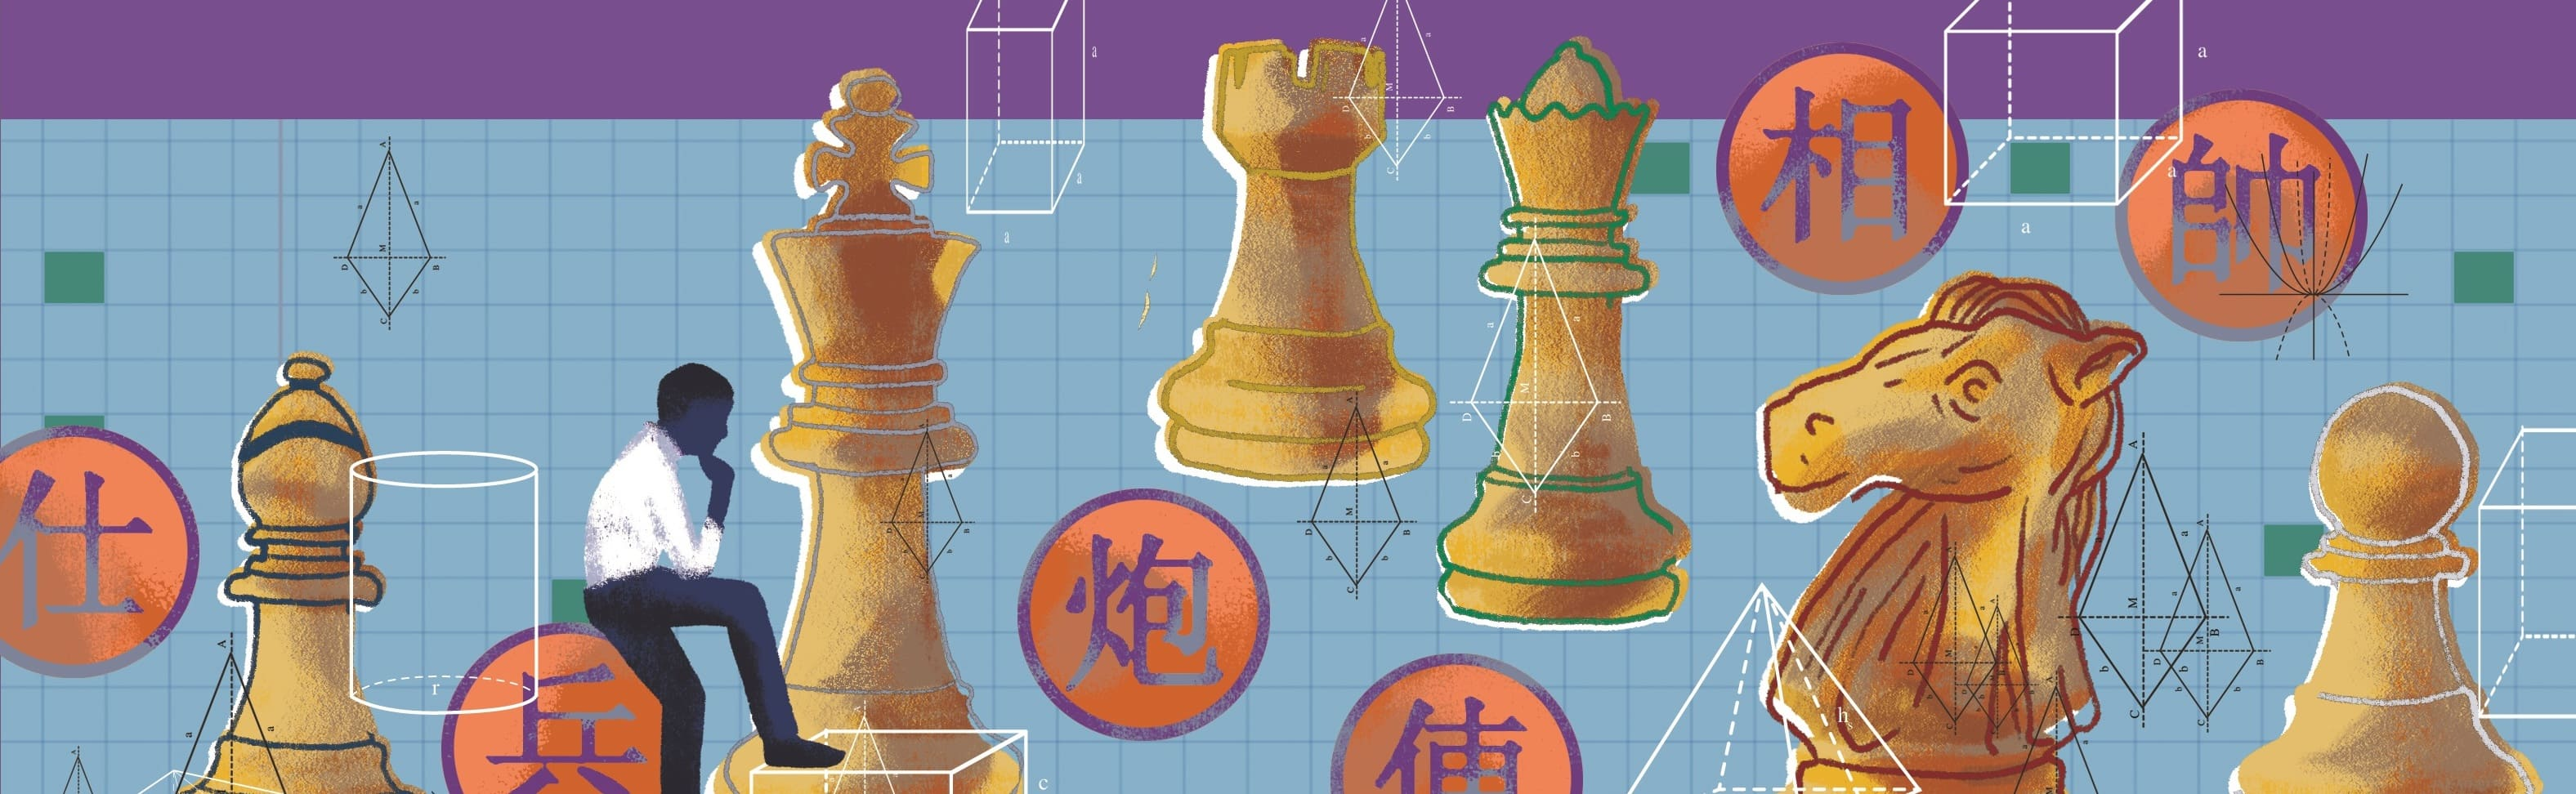
\includegraphics[width=19.3cm]{../bannergocco}}}
\AddToShipoutPicture*{\put(96,525){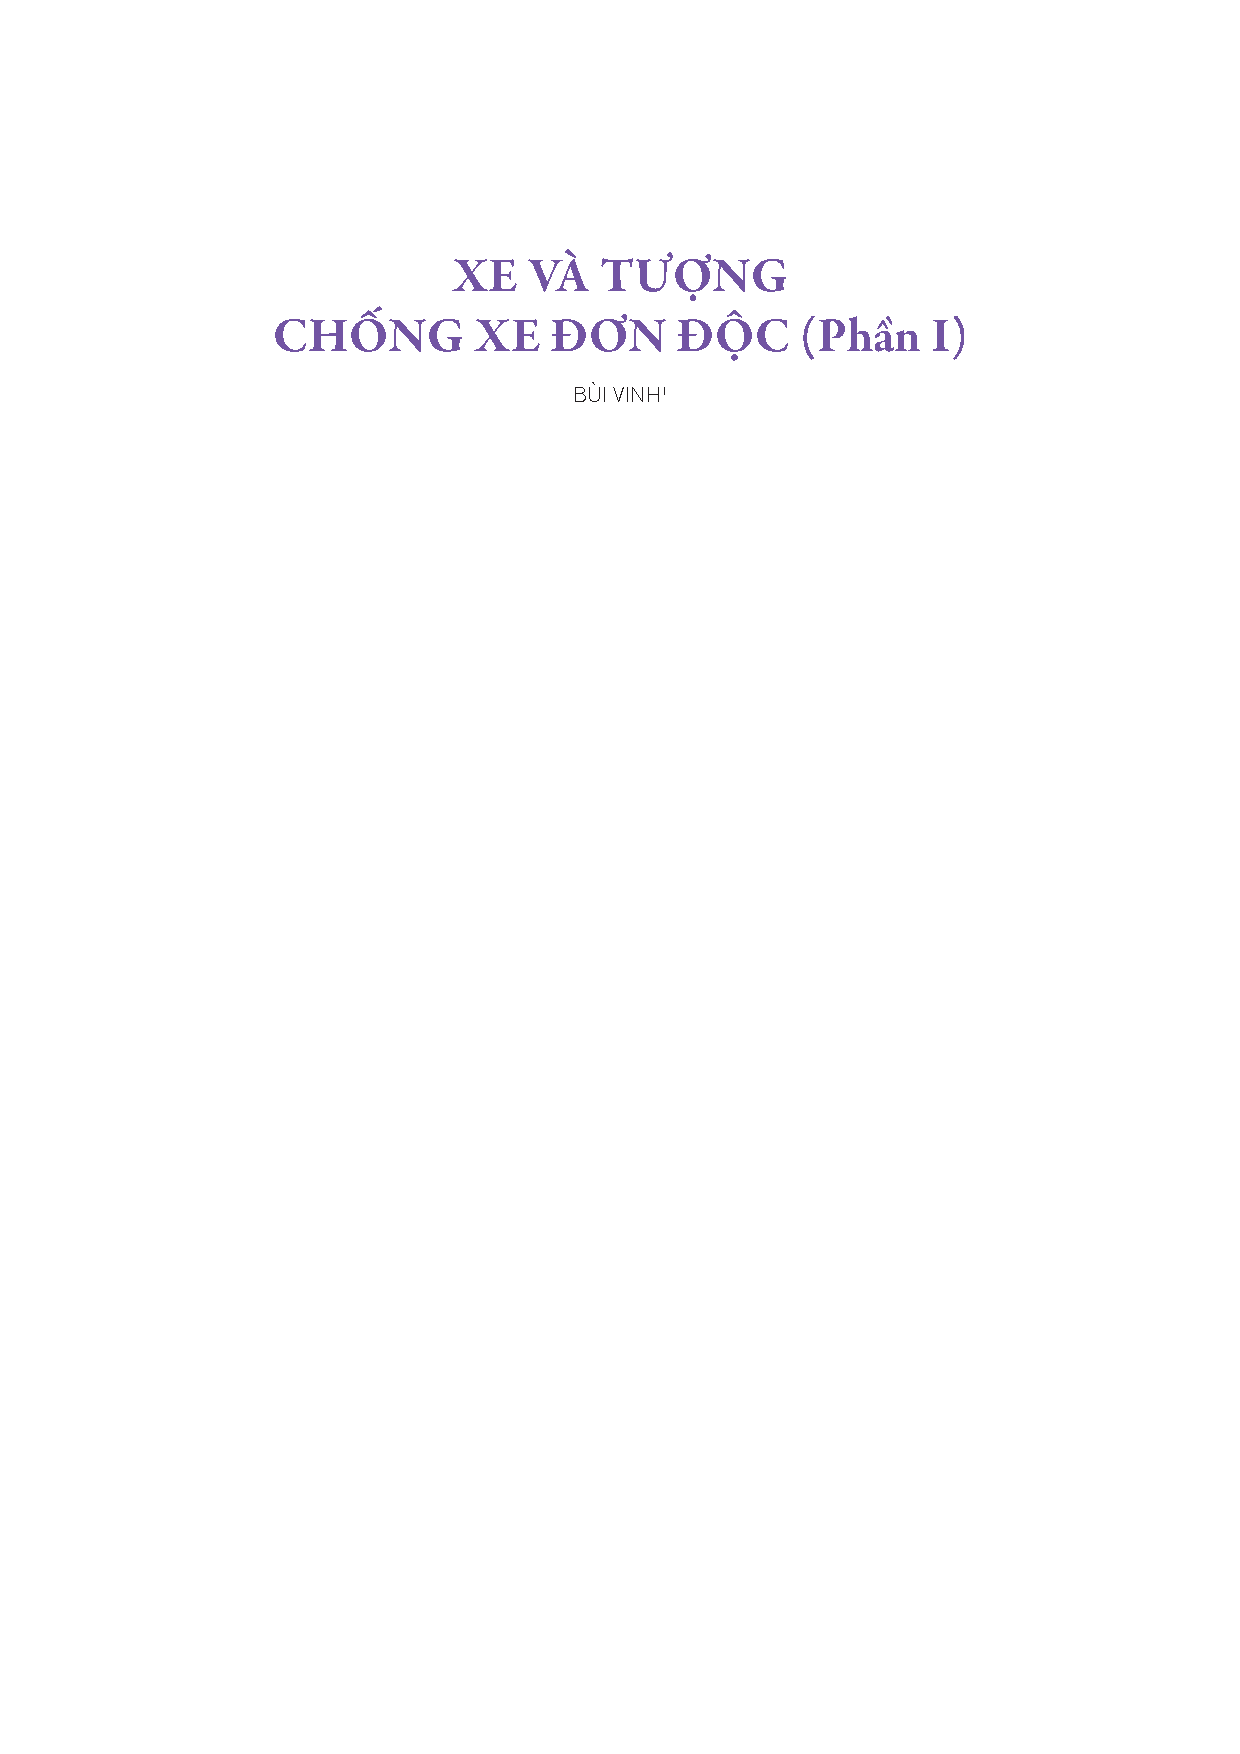
\includegraphics[scale=1]{../tieude.pdf}}} 
\centering
\endgroup

\vspace*{185pt}

\begin{multicols}{2}
	Lý thuyết cờ tàn cơ bản đều cho rằng xe và tượng chống xe không có tốt đều được coi là hòa cờ cơ bản. Tuy nhiên thực tế thi đấu cho thấy khả năng hòa cờ cho bên yếu không nhiều. Bên yếu cần phải chơi rất chính xác nếu muốn gỡ hòa.
	Trong bài học hôm nay, chúng tôi xin trình bày một số tình huống cơ bản 
	\vskip 0.1cm
	\textbf{\color{gocco}A.	Philidor}
	\begin{center}
		\newgame
		\fenboard{3k4/4r3/3K4/3B4/8/8/8/5R2 b Q - 0 1}
		\scalebox{0.85}\showboard
		\vskip 0.1cm
		\textit{\small\color{gocco}Hình $1$. Trắng đi trước thắng, $1749$.}
	\end{center}
	\textbf{\color{gocco}$\pmb{1}$.Xf$\pmb{8}$+ Xe$\pmb{8}$ $\pmb{2}$.Xf$\pmb{7}$ Xe$\pmb{2}$ $\pmb{3}$.Xh$\pmb{7}$} (Hình $2$) [Một nước đi chờ đợi]
	\vskip 0.1cm
	\textbf{\color{gocco}$\pmb{3}$...Xe$\pmb{1}$ $\pmb{4}$.Xb$\pmb{7}$! Xc$\pmb{1}$} [$4$...Vc$8$ $5$.Xa$7$ Xb$1$ $6$.Xh$7$! 
	\vskip 0.1cm
	$6$...Vb$8$ $7$.Xh$8$+ Va$7$ $8$.Xa$8$+ Vb$6$ $9$.Xb$8$+ Va$5$ $10$.Xxb$1$]
	\vskip 0.1cm
	\textbf{\color{gocco}$\pmb{5}$.Tb$\pmb{3}$!!} 
	\begin{center}
		\newgame
		\fenboard{2k5/7R/3K4/3B4/8/8/8/1r6 b Q - 0 1}
		\scalebox{0.85}\showboard
		\vskip 0.1cm
		\textit{\small\color{gocco}Hình $2$.}
	\end{center}
	\begin{center}
		\newgame
		\fenboard{3k4/1R6/3K4/8/8/1B6/8/2r5 b Q - 0 1}
		\scalebox{0.85}\showboard
		\vskip 0.1cm
		\textit{\small\color{gocco}Hình $3$.}
	\end{center}
	\textit{Kỹ thuật giành chiến thắng cơ bản của bên có tương là tìm cách ép vua đối phương xuống hàng ngang số $8,1$ hoặc cột a,h. Sau đó phối hợp giữa xe và tượng thực hiện vừa che chắn cho vua khỏi các nước chiếu của xe đối bằng tượng trong khi đó dùng xe đe dọa chiếu hết.}
	\vskip 0.1cm
	\textbf{\color{gocco}$\pmb{5}$...Xc$\pmb{3}$ $\pmb{6}$.Te$\pmb{6}$! Xd$\pmb{3}$+ $\pmb{7}$.Xd$\pmb{5}$} [Tượng trắng che chắn cho vua]
	\vskip 0.1cm
	$7$...Xc$3$ $8$.Xd$7$+ Vc$8$ $9$.Xh$7$ Vb$8$ $10$.Xb$7$+ Vc$8$ $11$.Xb$4$ Vd$8$ $12$.Tc$4$!! (Hình $4$). Trắng dùng Tượng ngăn cản xe đối phương phòng thủ ở ô c$8$.
	\begin{center}
		\newgame
		\fenboard{3k4/8/3K4/8/1RB5/2r5/8/8 b Q - 0 1}
		\scalebox{0.85}\showboard
		\vskip 0.1cm
		\textit{\small\color{gocco}Hình $4$.}
	\end{center}
	Trắng đe dọa chiếu hết ở nước tiếp theo
	\vskip 0.1cm
	\textbf{\color{gocco}$\pmb{12}$...Vc$\pmb{8}$} [$12$...Ve$8$ $13$.Xb$8\#$]
	\vskip 0.1cm
	\textbf{\color{gocco}$\pmb{13}$.Te$\pmb{6}$+ Vd$\pmb{8}$ $\pmb{14}$.Xb$\pmb{8}$+}
	\vskip 0.1cm
	\textbf{\color{gocco}Lolli}
	\begin{center}
		\newgame
		\fenboard{2k5/3r4/2K5/2B5/8/8/8/4R3 b Q - 0 1}
		\scalebox{0.85}\showboard
		\vskip 0.1cm
		\textit{\small\color{gocco}Hình $5$. Trắng đi trước thắng, $1763$.}
	\end{center}
	Trong rất nhiều trường hợp mặc dù xe đen cũng phòng thủ từ phía sau hoặc bên sườn, tuy nhiên bên mạnh cũng vẫn thắng.
	\vskip 0.1cm
	\textbf{\color{gocco}$\pmb{1}$.Xe$\pmb{8}$+ Xd$\pmb{8}$ $\pmb{2}$.Xe$\pmb{7}$ Xd$\pmb{2}$} [Nếu $2$...Xh$8$ $3$.Td$6$ Vd$8$ $4$.Xa$7$ Ve$8$ $5$.Xa$8+$; Nếu $2$...Xg$8$ $3$.Td$6$ Vd$8$ $4$.Xe$6$! (Hình $6$)
	\begin{center}
		\newgame
		\fenboard{3k2r1/8/2KBR3/8/8/8/8/8 b Q - 0 1}
		\scalebox{0.85}\showboard
		\vskip 0.1cm
		\textit{\small\color{gocco}Hình $6$.}
	\end{center}
	$4$...Vc$8$ ($4$...Xh$8$ $5$.Te$5$ Xf$8$ $6$.Tg$7$! Trắng giam xe đen ở hàng ngang số $8$
	\begin{center}
		\newgame
		\fenboard{3k1r2/6B1/2K1R3/8/8/8/8/8 b Q - 0 1}
		\scalebox{0.85}\showboard
		\vskip 0.1cm
		\textit{\small\color{gocco}Hình $7$.}
	\end{center}
	$6$...Xg$8$ $7$.Tf$6$+ Vc$8$ $8$.Xe$4$ Xf$8$ $9$.Tg$7$ Xg$8$ $10$.Xa$4$ Vb$8$ (\textit{$10$...Vd$8$ $11$.Xa$8$+}) $11$.Te$5$+ Vc$8$ $12$.Xa$8\#$) $5$.Xe$5$ Vd$8$ $6$.Tc$7$+ Vc$8$ $7$.Xa$5$ Xg$6$+ $8$.Td$6$+–]
	\vskip 0.1cm
	\textbf{\color{gocco}$\pmb{3}$.Xf$\pmb{7}$! Xd$\pmb{1}$} [$3$...Xd$8$ $4$.Te$7$ Xg$8$ $5$.Xf$5$ Vb$8$ $6$.Td$6$+ Vc$8$ $7$.Xa$5$]
	\vskip 0.1cm
	\textbf{\color{gocco}$\pmb{4}$.Xa$\pmb{7}$ Xb$\pmb{1}$} [$4$...Vb$8$ $5$.Xa$4$ Xc$1$ $6$.Xe$4$!]
	\begin{center}
		\newgame
		\fenboard{2k5/R7/2K5/8/8/B7/8/1r6 b Q - 0 1}
		\scalebox{0.85}\showboard
		\vskip 0.1cm
		\textit{\small\color{gocco}Hình $8$.}
	\end{center}
	$5$.Ta$3$!! 
	\vskip 0.1cm
	Nước cờ chìa khóa. Đen bị ``xung xoang" vì không có nước đi cho xe. 
	\vskip 0.1cm
	\textbf{\color{gocco}$\pmb{5}$...Xb$\pmb{3}$} [Phương án khác cũng không tốt hơn cho đen $5$...Vb$8$ $6$.Xe$7$ Va$8$ $7$.Xe$4$!! Xb$7$! $8$.Xe$5$ 
	\vskip 0.1cm
	Đen bị ``xung xoang" $8$...Xf$7$ ($8$...Xb$1$ $9$.Xa$5$+ Vb$8$ $10$.Td$6$+ Vc$8$ $11$.Xa$8$+) $9$.Xe$8$+ Va$7$ $10$.Tc$5$+ Va$6$ $11$.Xa$8$+ Trắng thắng]
	\begin{center}
		\newgame
		\fenboard{k7/1r6/2K5/4R3/8/B7/8/8 b Q - 0 1}
		\scalebox{0.85}\showboard
		\vskip 0.1cm
		\textit{\small\color{gocco}Hình $9$.}
	\end{center}
	\textbf{\color{gocco}$\pmb{6}$.Td$\pmb{6}$! Xc$\pmb{3}$+ $\pmb{7}$.Tc$\pmb{5}$}  
	\vskip 0.1cm
	Tượng trắng phối hợp với vua và xe. Tượng vừa thực hiện việc che chắn cho vua và tấn công vua đối phương.
	\begin{center}
		\newgame
		\fenboard{2k5/R7/2K5/2B5/8/2r5/8/8 b Q - 0 1}
		\scalebox{0.85}\showboard
		\vskip 0.1cm
		\textit{\small\color{gocco}Hình $10$.}
	\end{center}
	\textbf{\color{gocco}$\pmb{7}$...Xb$\pmb{3}$ $\pmb{8}$.Xc$\pmb{7}$+ Vb$\pmb{8}$} [$8$...Vd$8$ $9$.Xf$7$]
	\vskip 0.1cm
	\textbf{\color{gocco}$\pmb{9}$.Xe$\pmb{7}$ Va$\pmb{8}$ $\pmb{10}$.Xe$\pmb{4}$!} [$10$.Xe$8$+ Xb$8$ $11$.Xe$1$]
	\vskip 0.1cm
	\textbf{\color{gocco}$1\pmb{0}$...Xb$\pmb{7}$ $\pmb{11}$.Xa$\pmb{4}$+ Vb$\pmb{8}$ $\pmb{12}$.Td$\pmb{6}$+ Vc$\pmb{8}$ $\pmb{13}$.Xa$\pmb{8}$+} Trắng thắng
\end{multicols}